% Agile Orchestrators -- 2-minute Innovation Challenge pitch.
% Content: agile-orchestrators-2m-pitch.pptx (the team's short deck), plus the post-merge-docs
% skill. Look: same custom Rabobank design as ../agile-orchestrators-v5/main.tex (override of
% the latex-presentation default preamble). Speaker notes live in the source pptx and are
% copied into the exported main.pptx.
\documentclass[aspectratio=169,10pt]{beamer}
\usepackage[T1]{fontenc}
\usepackage[utf8]{inputenc}
\usepackage{lmodern}
\usepackage[scaled=0.92]{helvet}
\renewcommand{\familydefault}{\sfdefault}
\usepackage{amssymb}
\usepackage{tikz}
\usetikzlibrary{calc,positioning,arrows.meta,shapes.geometric,shapes.misc}

\graphicspath{{./images/}}

% ---------------------------------------------------------------- colours
\definecolor{raboNavy}{HTML}{000099}
\definecolor{raboBlue}{HTML}{0052FF}
\definecolor{raboLine}{HTML}{1C50D7}
\definecolor{raboOrange}{HTML}{FF6600}
\definecolor{raboGreen}{HTML}{03B463}
\definecolor{raboGrey}{HTML}{D9D9D9}
\definecolor{raboPanel}{HTML}{EDEDED}
\definecolor{raboLilac}{HTML}{E9E8F7}
\definecolor{raboPurple}{HTML}{7A2E8E}
\definecolor{raboInk}{HTML}{33334D}
\definecolor{raboMuted}{HTML}{8A8A99}
\definecolor{codeKey}{HTML}{FF8A3D}
\definecolor{codeText}{HTML}{E6E8FF}
\definecolor{codeMuted}{HTML}{9C9FE0}

% ---------------------------------------------------------------- beamer look
\setbeamertemplate{navigation symbols}{}
\setbeamersize{text margin left=0.8cm,text margin right=0.8cm}
\setbeamercolor{normal text}{fg=raboInk,bg=white}
\setbeamercolor{structure}{fg=raboBlue}
\setbeamercolor{alerted text}{fg=raboOrange}
\setbeamertemplate{itemize item}{\tikz[baseline=-0.55ex]\fill[raboOrange] (0,0) circle (1.5pt);}
\setbeamertemplate{itemize subitem}{\tikz[baseline=-0.55ex]\draw[raboBlue] (0,0) circle (1.2pt);}
\setlength{\leftmargini}{1.1em}
\hyphenpenalty=10000
\exhyphenpenalty=10000

\setbeamertemplate{frametitle}{%
  \vspace*{0.30cm}%
  {\color{raboBlue}\itshape\footnotesize\insertframesubtitle\par}%
  \vspace{0.5pt}%
  {\color{raboBlue}\itshape\fontsize{19}{21}\selectfont\insertframetitle\par}%
}

% Phase tracker (Prepare / Build / Close), drawn top right when \phaseno is 1, 2 or 3.
\def\phaseno{0}
\newcommand{\phasechev}[4]{% x, label, index, fill
  \ifnum#3=\phaseno
    \fill[#4] (#1,8.12) -- (#1+1.15,8.12) -- (#1+1.37,8.40) -- (#1+1.15,8.68) -- (#1,8.68)
      -- (#1+0.22,8.40) -- cycle;
    \node[text=white,font=\scriptsize\itshape\bfseries] at (#1+0.69,8.40) {#2};
  \else
    \fill[raboPanel] (#1,8.12) -- (#1+1.15,8.12) -- (#1+1.37,8.40) -- (#1+1.15,8.68) -- (#1,8.68)
      -- (#1+0.22,8.40) -- cycle;
    \node[text=raboMuted,font=\scriptsize\itshape] at (#1+0.69,8.40) {#2};
  \fi}

% Default background: page number bottom left, footer + logo bottom right.
\defbeamertemplate{background}{content}{%
  \begin{tikzpicture}
    \useasboundingbox (0,0) rectangle (16,9);
    \node[anchor=south east,inner sep=0] at (15.72,0.16)
      {
\includegraphics[height=0.70cm]{rabobank-logo}};
    \node[anchor=south east,text=raboBlue,font=\scriptsize\itshape,inner sep=0] at (15.02,0.24)
      {Agile Orchestrators \,\textperiodcentered\, Innovation Challenge};
    \node[anchor=south west,text=raboMuted,font=\tiny,inner sep=0] at (0.3,0.24)
      {\insertframenumber};
    \ifnum\phaseno>0
      \phasechev{11.05}{Prepare}{1}{raboOrange}
      \phasechev{12.36}{Build}{2}{raboGreen}
      \phasechev{13.67}{Close}{3}{raboNavy}
    \fi
  \end{tikzpicture}}
\setbeamertemplate{background}[content]

% Gradient ring used on the title and closing slides.
\newcommand{\connectorring}[3]{% centre x, centre y, radius
  \foreach \i in {0,...,59}{%
    \pgfmathsetmacro{\a}{215-\i*5.5}%
    \pgfmathtruncatemacro{\p}{100-\i*100/59}%
    \draw[line width=2.6pt,draw=raboOrange!\p!raboPurple]
      ($(#1,#2)+(\a:#3)$) arc[start angle=\a,end angle=\a-5.7,radius=#3];
  }%
  \draw[raboPurple!45,line width=0.5pt] ($(#1,#2)+(250:#3-0.28)$)
    arc[start angle=250,end angle=150,radius=#3-0.28];
}
\newcommand{\ringdot}[5]{% cx, cy, r, angle, label
  \pgfmathtruncatemacro{\q}{max(0,min(100,(215-#4)/3.3))}%
  \filldraw[fill=white,draw=raboOrange!\q!raboPurple,line width=1.3pt]
    ($(#1,#2)+(#4:#3)$) circle (0.17);
  \node[font=\tiny\itshape,text=raboInk,inner sep=1pt,anchor=#4+180] at ($(#1,#2)+(#4:#3+0.25)$) {#5};
}
% Title/closing layout: navy band, orange box, grey line, ring on the right.
\newcommand{\titlelayout}[4]{% band text, orange box text, grey line, ring script
  \begin{tikzpicture}
    \useasboundingbox (0,0) rectangle (16,9);
    \fill[raboOrange,rounded corners=1.5pt] (0.8,5.72) rectangle (1.02,5.94);
    \node[anchor=west,text=raboOrange,font=\small\bfseries,inner sep=0] at (1.15,5.83)
      {Innovation Challenge};
    \fill[raboNavy] (0,4.30) rectangle (9.9,5.45);
    \node[anchor=west,text=white,font=\fontsize{26}{28}\selectfont\itshape] at (0.8,4.86) {#1};
    \fill[raboOrange,rounded corners=5pt] (3.5,2.85) rectangle (9.9,4.10);
    \node[anchor=west,text=white,font=\normalsize\bfseries\itshape,text width=6.0cm,align=left]
      at (3.7,3.47) {#2};
    \node[anchor=north west,text=raboMuted,font=\scriptsize,text width=6.3cm,align=left]
      at (3.55,2.62) {#3};
    % thin line-art path leading into the ring
    \draw[raboLine,line width=0.7pt] (9.9,3.47) .. controls (10.6,3.47) and (10.4,4.2) .. (10.95,4.55);
    \fill[raboLine] (9.9,3.47) circle (2pt);
    \connectorring{12.55}{5.75}{2.05}
    \ringdot{12.55}{5.75}{2.05}{160}{Messaging}
    \ringdot{12.55}{5.75}{2.05}{112}{Email}
    \ringdot{12.55}{5.75}{2.05}{66}{Meeting notes}
    \ringdot{12.55}{5.75}{2.05}{20}{Documentation}
    \ringdot{12.55}{5.75}{2.05}{-26}{Project board}
    \ringdot{12.55}{5.75}{2.05}{-72}{Diagram tool}
    \node[align=center,font=\footnotesize,text=raboNavy] at (12.55,5.95)
      {\textbf{\large AI agent}\\[1pt] {\scriptsize AGILE ORCHESTRATORS}};
    \node[rotate=8,font=\small\itshape\bfseries,text=raboOrange] at (12.7,5.15) {#4};
    \node[anchor=south east,inner sep=0] at (15.6,0.35)
      {
\includegraphics[height=1.35cm]{rabobank-logo}};
  \end{tikzpicture}}

% ---------------------------------------------------------------- tikz styles
\tikzset{
  obox/.style={rounded corners=4pt,fill=raboOrange,text=white,align=center,
    font=\scriptsize,inner sep=3pt},
  gbox/.style={rounded corners=4pt,fill=raboGreen,text=white,align=center,
    font=\scriptsize,inner sep=3pt},
  nbox/.style={rounded corners=4pt,fill=raboNavy,text=white,align=center,
    font=\scriptsize,inner sep=3pt},
  wbox/.style={rounded corners=4pt,fill=white,draw=raboGrey,line width=0.8pt,text=raboInk,
    align=center,font=\scriptsize,inner sep=3pt},
  panel/.style={rounded corners=9pt,fill=raboPanel},
  line/.style={raboLine,line width=0.7pt},
  arr/.style={raboLine,line width=0.8pt,-{Stealth[length=2.2mm]}},
  htitle/.style={font=\small\itshape,text=raboBlue,anchor=north west,inner sep=0},
  body/.style={font=\scriptsize,text=raboInk,anchor=north west,inner sep=0,align=left},
  bubbleme/.style={fill=raboNavy,text=white,rounded corners=6pt,font=\small,inner sep=6pt,
    align=left},
  bubbleai/.style={fill=raboPanel,text=raboInk,rounded corners=6pt,font=\small,inner sep=6pt,
    align=left},
  callout/.style={fill=raboLilac,rounded corners=6pt,font=\scriptsize\itshape,text=raboNavy,
    inner sep=6pt,align=left,anchor=north west},
}
\newcommand{\sk}[1]{\texttt{#1}}

% One step of a phase: grey column, number on the line-art path, step, skill pill, context.
% x, width, number, step, skill, context, pill style
\newcommand{\stepcol}[7]{%
  \fill[panel] (#1,4.45) rectangle (#1+#2,1.55);
  \filldraw[fill=white,draw=raboLine,line width=0.9pt] (#1+#2/2,4.95) circle (0.27);
  \node[font=\scriptsize\bfseries\itshape,text=raboBlue] at (#1+#2/2,4.95) {#3};
  \node[font=\small\bfseries,text=raboNavy,align=center,text width=#2 cm-0.3cm]
    at (#1+#2/2,3.95) {#4};
  \node[#7,font=\scriptsize\ttfamily,minimum width=#2 cm-0.5cm,minimum height=0.55cm]
    at (#1+#2/2,3.2) {#5};
  \node[font=\tiny\itshape,text=raboMuted,anchor=north west,inner sep=0] at (#1+0.25,2.7)
    {Context it uses};
  \node[body,text width=#2 cm-0.5cm] at (#1+0.25,2.38) {#6};
}
% Thin line-art path behind the step numbers.
\newcommand{\steppath}[1]{% end x
  \draw[line] (0.1,4.95) -- (#1,4.95);
  \fill[raboLine] (0.1,4.95) circle (1.8pt);
  \draw[arr] (#1-0.4,4.95) -- (#1,4.95);
}


% Inline skill pill that wraps with the surrounding text.
\newcommand{\pill}[2]{\tikz[baseline=(p.base)]\node[#1,font=\tiny\ttfamily,inner sep=2.5pt,
  rounded corners=3pt] (p) {#2};}

\begin{document}

% ================================================================ 1 title
{\setbeamertemplate{background}{\titlelayout{Agile Orchestrators}
   {AI agents for Agile\\ ways of working}
   {Adam Alansary \textperiodcentered\ Cedric Baron \textperiodcentered\ Jasper Krebbers
    \textperiodcentered\ Theun van Vliet \textperiodcentered\ Stefan Wachmann}
   {Scrum, orchestrated}}
 \begin{frame}[plain]\mbox{}\end{frame}}

% ================================================================ 2 challenge
\begin{frame}[t]{The challenge}{Why we started}
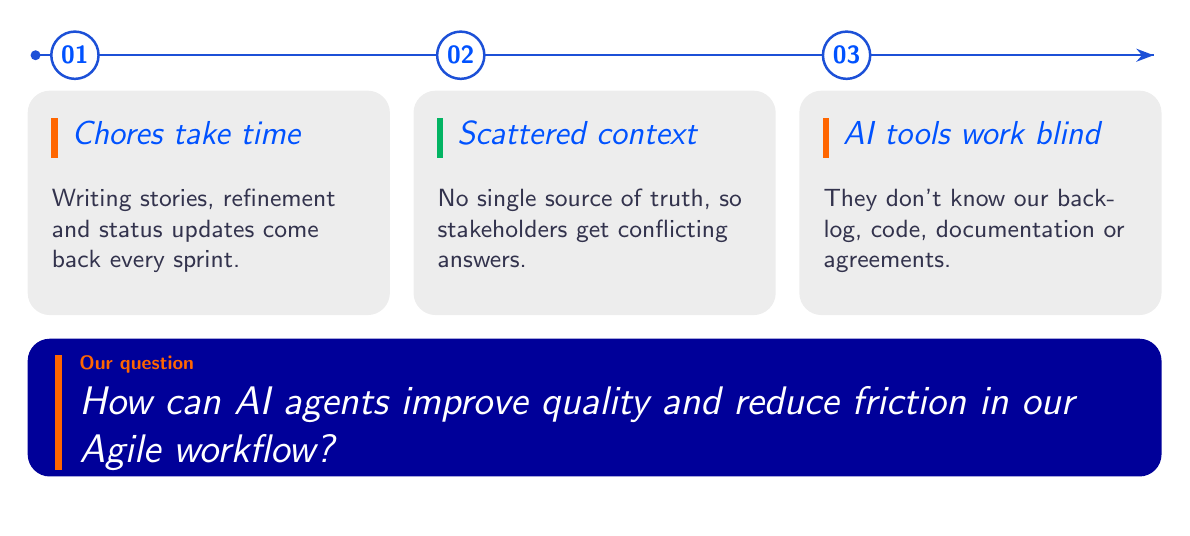
\begin{tikzpicture}
  \useasboundingbox (0,0) rectangle (14.4,6.1);
  % line-art path through the three numbers
  \draw[line] (0.1,5.75) -- (14.3,5.75);
  \fill[raboLine] (0.1,5.75) circle (1.8pt);
  \draw[arr] (13.9,5.75) -- (14.3,5.75);
  \foreach \x/\c/\n/\h/\d in {
    0/raboOrange/01/Chores take time/{Writing stories, refinement and status updates come
      back every sprint.},
    4.9/raboGreen/02/Scattered context/{No single source of truth, so stakeholders get
      conflicting answers.},
    9.8/raboOrange/03/AI tools work blind/{They don't know our backlog, code, documentation
      or agreements.}}{
    \fill[raboPanel,rounded corners=8pt] (\x,5.3) rectangle (\x+4.6,2.45);
    \filldraw[fill=white,draw=raboLine,line width=0.9pt] (\x+0.6,5.75) circle (0.3);
    \node[font=\small\bfseries\itshape,text=raboBlue] at (\x+0.6,5.75) {\n};
    \fill[\c] (\x+0.3,4.95) rectangle (\x+0.38,4.45);
    \node[htitle,font=\large\itshape] at (\x+0.55,4.92) {\h};
    \node[body,text width=3.95cm,font=\small] at (\x+0.3,4.05) {\d};
  }
  \fill[raboNavy,rounded corners=8pt] (0,2.15) rectangle (14.4,0.4);
  \node[anchor=north west,inner sep=0,font=\scriptsize\bfseries,text=raboOrange] (qlabel)
    at (0.65,1.94) {Our question};
  \node[anchor=north west,inner sep=0,font=\fontsize{13.5}{17}\selectfont\itshape,text=white,
    text width=13.4cm,align=left] (qtext) at (0.65,1.54)
    {How can AI agents improve quality and reduce friction in our Agile workflow?};
  % accent bar spans exactly from the label's top to the question's bottom
  \fill[raboOrange] (0.35,0 |- qlabel.north) rectangle (0.43,0 |- qtext.south);
\end{tikzpicture}
\end{frame}

% ================================================================ 3 what we built
\begin{frame}[t]{What we built}{A sprint at Tulip Bank}
\begin{tikzpicture}
  \useasboundingbox (0,0) rectangle (14.4,6.1);
  \node[body,text width=14.2cm,font=\small\itshape,text=raboNavy] at (0,6.0)
    {We ran a sprint at Tulip Bank, a fictional bank that works the way Rabobank does. Our AI
     agent could reach the board, wiki, chat, meeting notes and Miro.};
  \node[anchor=north west,inner sep=0,font=\scriptsize\bfseries,text=raboMuted] at (0,5.0)
    {\textcolor{raboOrange}{\large 13} \;Skills: work instructions for the agent, kept in the
     repository};
  \foreach \y/\c/\s/\ph/\h/\pills in {
    4.4/raboOrange/obox/Prepare/Business goal to planned sprint/{\pill{obox}{create-epic}
      \pill{obox}{create-features} \pill{obox}{create-pbis} \pill{obox}{refinement-session}
      \pill{obox}{sprint-planning}},
    2.95/raboGreen/gbox/Build/{Code, pull requests, findings and docs}/{\pill{gbox}{work-on-pbi}
      \pill{gbox}{verify-publish-pr} \pill{gbox}{review-pr} \pill{gbox}{log-finding}
      \pill{gbox}{post-merge-docs}},
    1.5/raboNavy/nbox/Close/{Wrap-up, sprint review and retro}/{\pill{nbox}{ending-the-sprint}
      \pill{nbox}{create-sprint-overview} \pill{nbox}{create-retrospective}}}{
    \fill[raboPanel,rounded corners=7pt] (0,\y) rectangle (7.6,\y-1.3);
    \fill[\c] (0,\y) -- (1.55,\y) -- (1.85,\y-0.65) -- (1.55,\y-1.3) -- (0,\y-1.3) -- cycle;
    \node[text=white,font=\small\bfseries\itshape] at (0.85,\y-0.65) {\ph};
    \node[anchor=north west,inner sep=0,font=\small\bfseries,text=raboNavy] at (2.1,\y-0.17)
      {\h};
    \node[anchor=north west,inner sep=0,text width=5.4cm,align=left,
      font={\fontsize{5}{12}\selectfont}] at (2.1,\y-0.55) {\pills};
  }
  \node[anchor=north east,inner sep=0] (img) at (14.4,5.05)
    {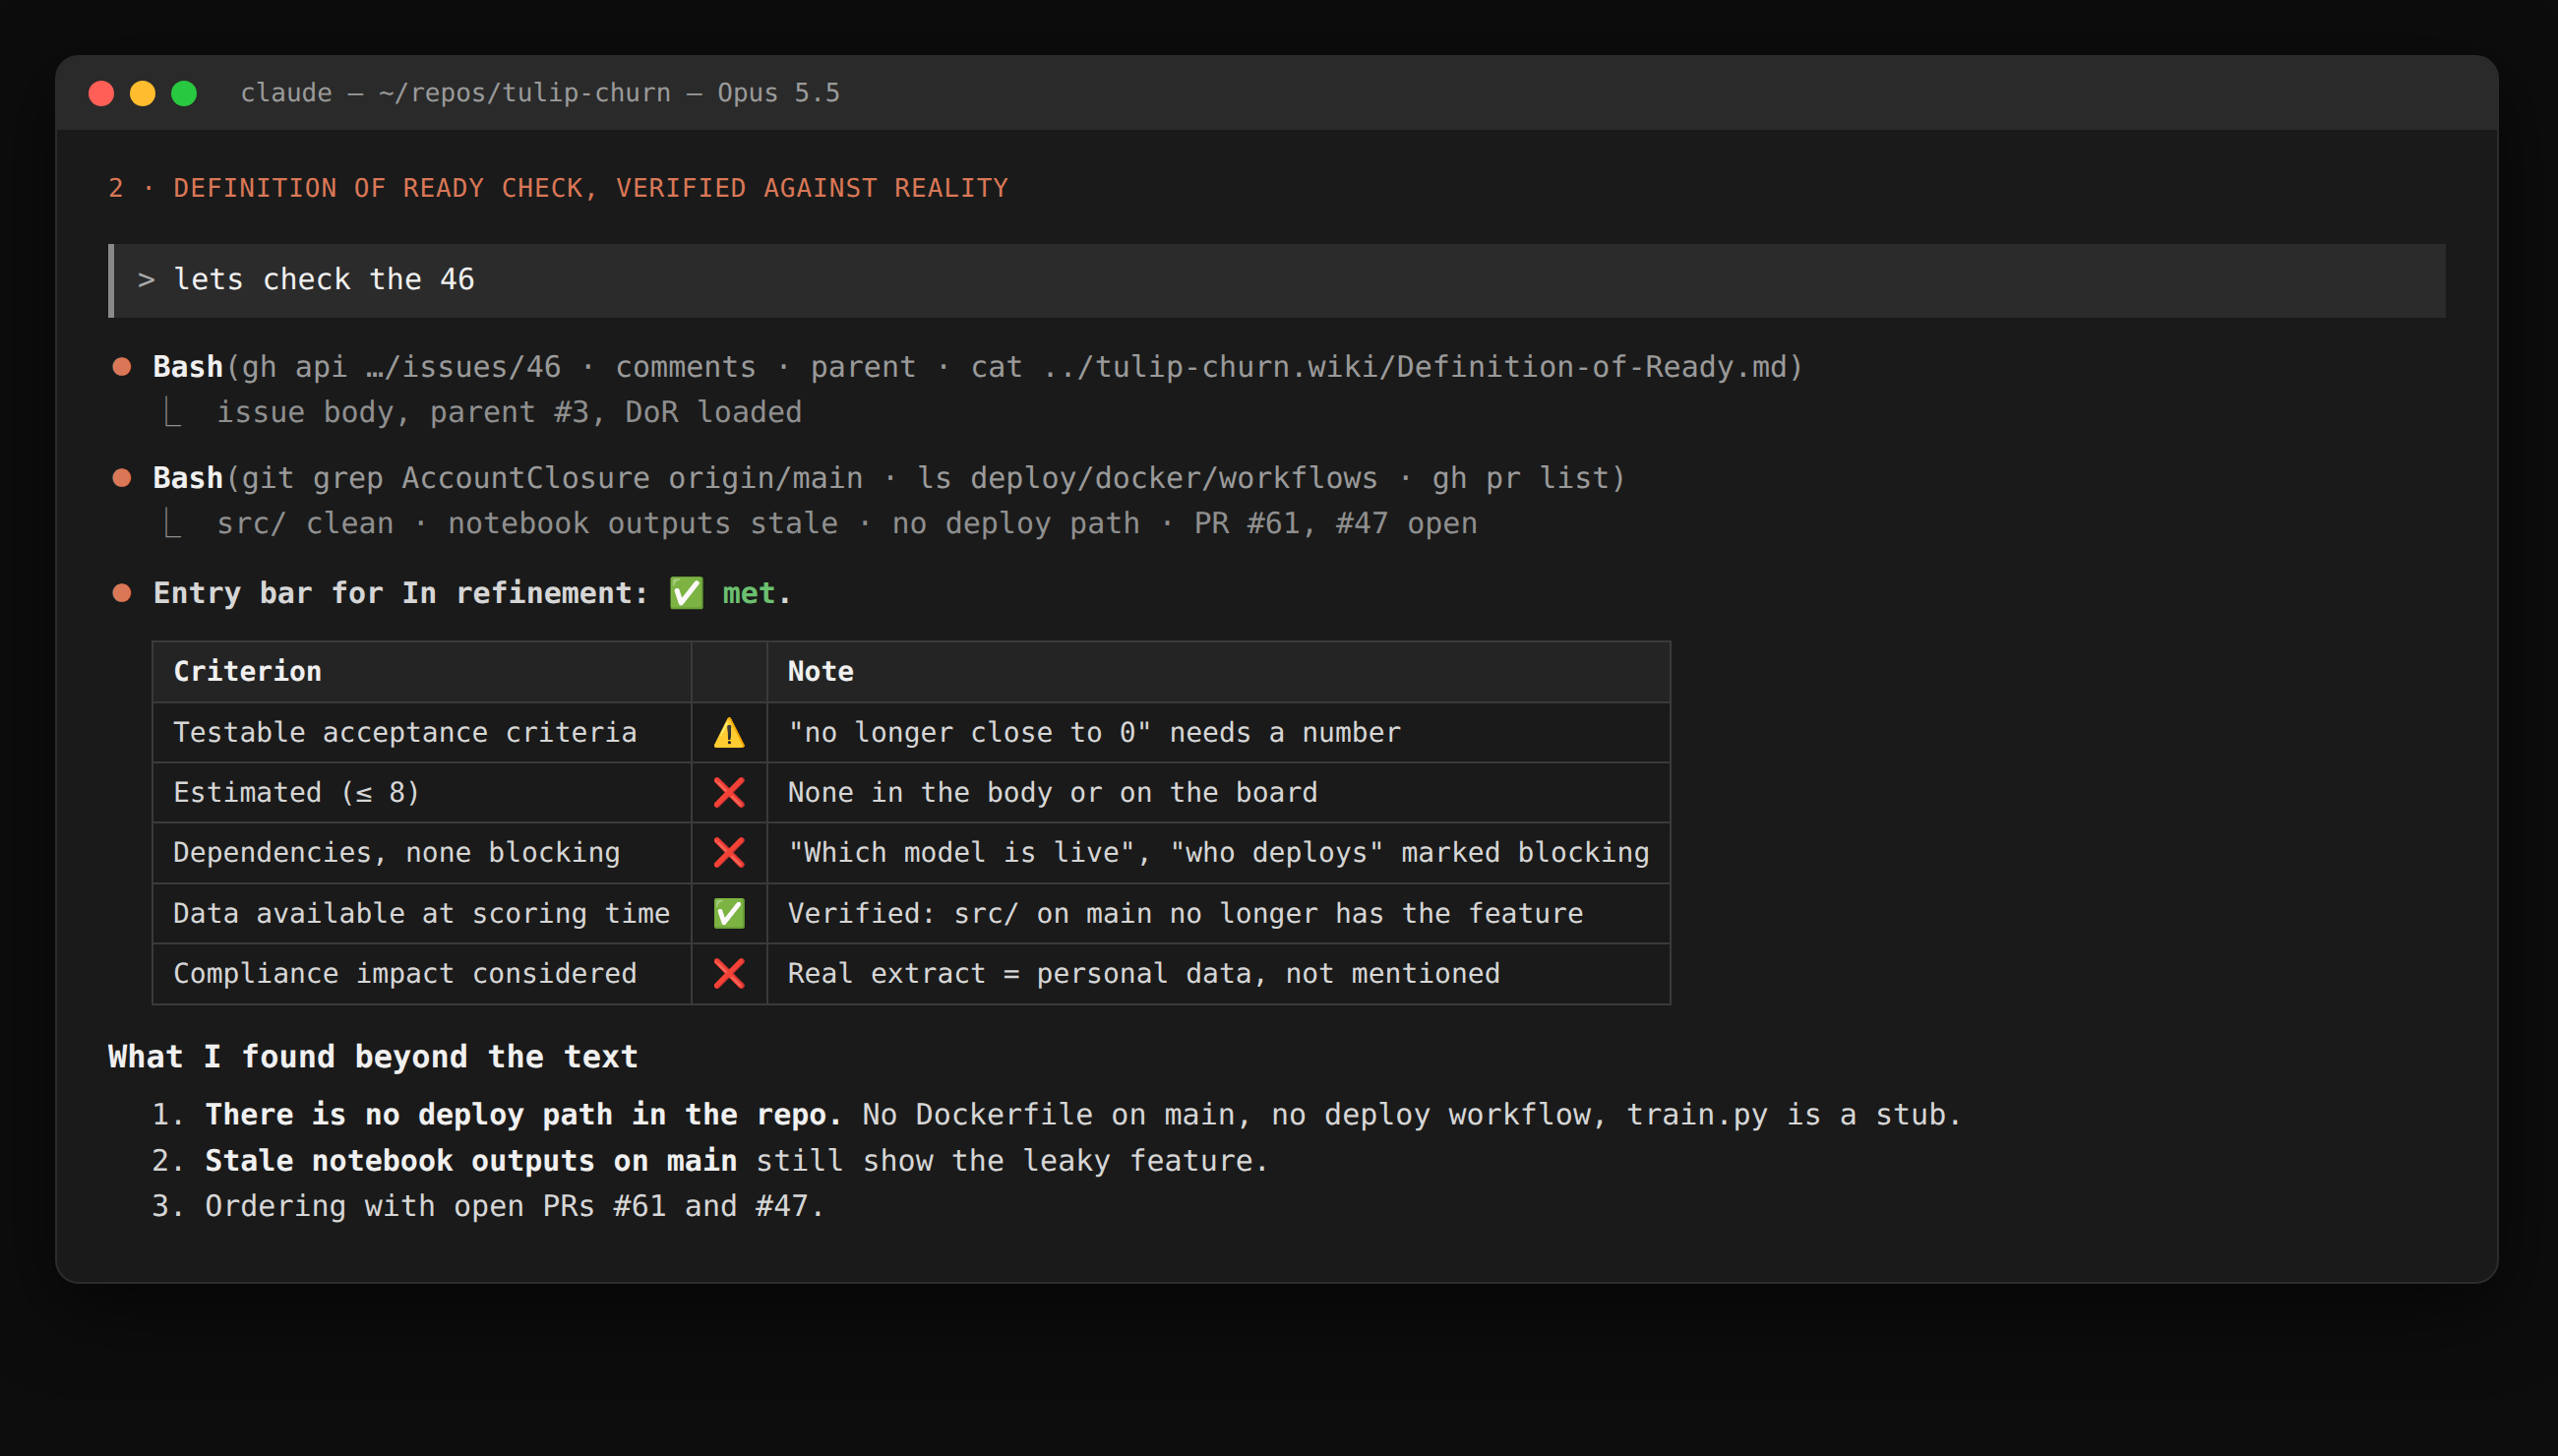
\includegraphics[width=6.3cm]{refinement-terminal}};
  \draw[line] (8.1,1.2) -- (8.1,0.35);
  \node[anchor=north west,inner sep=0,text width=5.9cm,align=left,font=\small\itshape,
    text=raboBlue] at (8.35,1.2)
    {In refinement, the agent checks the PBI against the code and finds hidden blockers.};
\end{tikzpicture}
\end{frame}

% ================================================================ 4 learned / ask
\begin{frame}[t]{What we learned and what we ask}{Lessons that carry over}
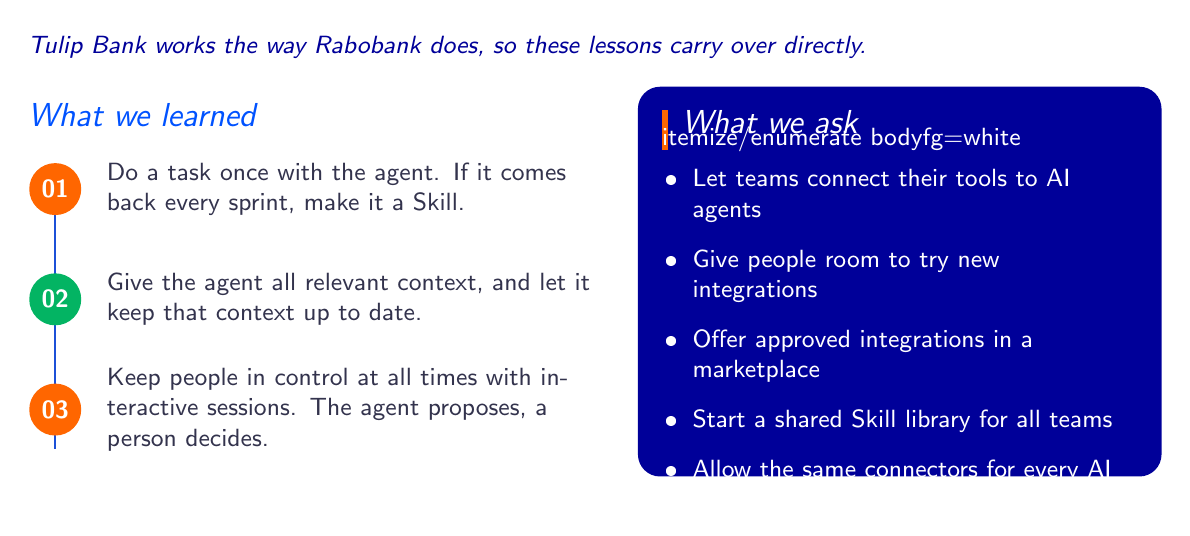
\begin{tikzpicture}
  \useasboundingbox (0,0) rectangle (14.4,6.1);
  \node[body,font=\small\itshape,text=raboNavy] at (0,6.0)
    {Tulip Bank works the way Rabobank does, so these lessons carry over directly.};
  \node[htitle,font=\large\itshape] at (0,5.15) {What we learned};
  \draw[line] (0.35,4.2) -- (0.35,0.75);
  \foreach \c/\t [count=\i] in {
    raboOrange/{Do a task once with the agent. If it comes back every sprint, make it a Skill.},
    raboGreen/{Give the agent all relevant context, and let it keep that context up to date.},
    raboOrange/{Keep people in control at all times with interactive sessions. The agent
      proposes, a person decides.}}{
    \pgfmathsetmacro{\y}{4.05-(\i-1)*1.4}
    \fill[\c] (0.35,\y) circle (0.33);
    \node[text=white,font=\small\bfseries] at (0.35,\y) {0\i};
    \node[anchor=west,inner sep=0,text width=6.2cm,align=left,font=\small,text=raboInk]
      at (1.0,\y) {\t};
  }
  \fill[raboNavy,rounded corners=8pt] (7.75,5.35) rectangle (14.4,0.4);
  \fill[raboOrange] (8.05,5.05) rectangle (8.13,4.55);
  \node[htitle,font=\large\itshape,text=white] at (8.3,5.05) {What we ask};
  \node[body,text width=5.9cm,font=\small,text=white] at (8.05,4.85) {%
    \setbeamercolor{itemize/enumerate body}{fg=white}\color{white}%
    \begin{itemize}\setlength{\itemsep}{5pt}
      \item Let teams connect their tools to AI agents
      \item Give people room to try new integrations
      \item Offer approved integrations in a marketplace
      \item Start a shared Skill library for all teams
      \item Allow the same connectors for every AI agent
    \end{itemize}};
\end{tikzpicture}
\end{frame}

\end{document}
